% Metódy inžinierskej práce

\documentclass[10pt,twoside,slovak,a4paper]{article}

\usepackage[slovak]{babel}
%\usepackage[T1]{fontenc}
\usepackage[IL2]{fontenc} 
\usepackage[utf8]{inputenc}
\usepackage{graphicx}
\usepackage{url} 
\usepackage{hyperref} 

\usepackage{cite}
%\usepackage{times}

\pagestyle{headings}

\title{Názov\thanks {Semestrálny projekt v predmete Metódy inžinierskej práce, ak. rok 2022/23, vedenie: Zuzana Špitálová}} % meno a priezvisko vyučujúceho na cvičeniach

\author{Mariia Lytvynova\\[2pt]
	{\small Slovenská technická univerzita v Bratislave}\\
	{\small Fakulta informatiky a informačných technológií}\\
	{\small \texttt{xlytvynova@stuba.sk}}
	}

\date{\small 6. november 2022} % upravte



\begin{document}

\maketitle

\begin{abstract}

Už viac ako 50 rokov ľudia hrajú v počitačové hri. Vyzerá tak, že v posledných rokoch si čoraz väčší priestor získava hranie hier na počítačoch, mobiloch a hracích konzolách.  Dnes adaptívne užívateľské modelovanie zaujíma viac ľudí, ved toto pomôže zvýšiť popularitu a využivanie počítačových hier. Keď hráč má slabší zvyky, tak podľaňho to je viac komplikovano. Aj taka istá situácia, keď podľa hráča hra je ľahká, tak potom sa vzdá. Adaptívne užívateľské modelovanie má pekný potenciál, aby človek začal viac zaujímať sa o hre a zároveň inšpiruje hrača pokračovať dalej. Rôzne typy potrebujú rôzne prístupy do prispôsobenia. V tomto článku búde rozprávať o takých prípadoch ak adaptovanie trasy, využívaniu prekážok alebo odmien. 
\end{abstract}



\section{Úvod}

Dnes počítačové hry stali obyčajným spôsobom tráviť čas. Rychlé šoférovanie a driftovanie sú dôvody, prečo automobilové závodné hry zaujímajú ľudia. Teraz spoločnosti súťažia o tom, ako urobiť adaptívne užívateľské modelovanie v automobilových závodných hrách. Hodnotenie skúseností hráča aj adaptívne užívateľské modelovanie zvýšia zaujímavosti hráčov. Schopnosť šoférovania a požiadavky hry potrebuje byť vyvážené. Pocit, ked´ zvladnul prejsť úroveň inšpiruje hráča pokračovať ďalej. Podľa pomeru schopnosti a požiadaviek sú štyri prípady []. Po prvé, obaja sú vysoké. Hráč má pekné skusenosti, ale aj požiadavky sú vysoké, a preto má možnosť na sebazdokonaľovanie. Dalej môže byť iný prípad, keď hráč má vysoké schopnosti, ale požiadavky zodpovedajú. Preto začína nudiť. Naopak je, ked´ má nizké skúseností a výzvy sú vzsoké. Nemôže prejsť na iny úroveň, a preto sa vzda.
Cieľom tohto článku je opísať rôzne spôsoby adaptovania počítačových zavodnych hrach pre hráča. Prvým spôsobom je spôsob odmen a prekážok.  Ďalej je  adaptovanie trasy podľa skúseností a slabosej hráča.

\section{Prvá časť} \label{prvá časť}

Každý hráč má rôzne schopnosti a slabosti. Problém v adaptivnom užívateľskom modelovaný je urobiť tak, aby všetky hráčy citili, že hra je spravodlivá. Ked´ hra začína zrejmé vyrovnávať, tak hračovský zaujem zniší.  Hráčy s lepšimy skúsenosťami citia, že ich schopnosti nie je dôležitý. Slabé hráčy myslia, že ich schopnosti znamenajú nič. Preto je dôležité urobiť tak, aby hráčy nerozumeli, či hra využíva adaptovanie.
Faktory, ktoré ovplyvnia na rezultaty hry:
\begin{itemize}
\item Vzdialenosť medzi automobilmi. Bez ohľadu na skusenosty a vysledok, ked´ sú blízko, tak hračy cítia duch súperenia.
\item Možnosť pozerať ine auto. Pre všetkých možnosť pozerať na súpera pomáha zvýšiť zaujem a pocit revality. Ak vzdialenosť je veľká a hráč nemôže pozerať na súpera, tak zmenší zaujem.
\item Zmena vedúceho pretekára. Prebehnutie roly pretekára pomáha udržať zaujem.
\end{itemize}
Vyváženie hráčov založené na týchto dôležitých faktorach. 
	Vyvažovacie mechanizmy založené na asistencii:
\begin{enumerate}
\item Rýchlosť. Zmena rýchlosti pomocou sčitania alebo odpočitania založené na odmenu alebo prekážku od -5 míľ / h do +5 míľ / h.
\item Zrýchlenie. Zrýchlenie sa nastavuje manipuláciou s parametrom airFriction automobilu pomocou empiricky stanovenej konštanty vynásobení úrovňou asistencie. Úroveň -5 značí, že auto potrebovalo 1.5x času, aby dosiahnuť maximálnu rýchlosť. Ked´ +5 - potrebuje 0.75x.
\item Riadenie. Hra začína porovnávať smer cesty a vypočíta chybu riadenia. Riadenie upravené o sumu primeranú chybe a úrovňou (od -5 do +5). +5  ako odmena, -5 ako prekážka.
\end{enumerate}
Dôsledkamy sú 10 urovňy možných prispôsobení: 5 odmen a 5 prekážok. 
	Algoritmy prispôsobenia:
\begin{itemize}
\item Realtime100. Tento algorithm kontroluje vzdialenosť medzi automobilmi. Ak je vyššia ako 1 meter, tak začínajú fungovať odmeny a prekážky. Napríklad, ak vzdialenosť je 1-100 metrov, tak lepši hráč ziska -1 úroveň prekážky, a horší - +1 úroveň odmeny.
\item Realtime40. Taká istá schema, len pre každý 40 metrov. To je viac rýchlejší a agresívny spôsob prispôsobenia. Lepšie využívať v krátkych závodoch.
\item Rolling. Hlavný nástroj – čas. Všetky odmeny a prekážky hráč môže získať len o 50 sekúnd, ale aj trvať to búdu viac času. Odmeny a prekážky búdu fungovať aj vtedy, keď podmienka splnenia prispôsobenia už nie je aktualná.
\item MaxDistance. Tento algoritm využiva Realtime100, ale skončí, ked´ vzdiaelnosť medzi automobilmi je 50 alebo menše metrov. Pomáha vyrovnávať hračov, ale ne prekáža, ked´ vzdialenosť je malá.
\end{itemize}

\paragraph{Výsledky}
Všetky účastníci absolvovali 8 pretekov pre dve osoby (jeden z nich bol simulovaný vodič). Účastníci boli rozdelené na 2 skupiny: odborníci a nováčici.
Výhry a straty
94.6\% odborníkov vyhrali závody áut a len 7.3\% z nováčikov.  Výsledky ukázané v Figure 1. Len 2 algoritmy pomohli nováčkam vyhrať, ešte 3 dovolili stratiť odborníčam. 
\begin{figure*}[tbh]
\centering
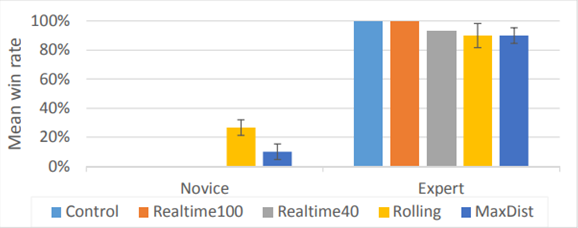
\includegraphics[scale=0.7]{figure1.png}
\caption{Figura 1. Výhry a straty}
\end{figure*}

\section{Druhá časť} \label{druha časť}

Adaptovanie trasy je komplikovaná úloha. Predovšetkým trasa musí byť rozdelená na niekoľko časti, tak aby každá časť obsahovala by len jeden typ cesty (priama, zákruta, chicane a t.d.). Dôležitým je te, aby obe strany cesty boli by ohradeny (hráč nemôže urobiť skratku). Výhoda tohto metoda je te, že algoritmus môže  urobiť 3 veci:
\begin{itemize}
\item Nechať trasu ako je, ak pre hráča to lepšie.
\item Urobiť ľahšiu, ak pre hráča to je komplikovaná.
\item Urobiť komplikovanejšiu, ak hráč má veľky skusenosti.
\end{itemize}
\paragraph{Algoritmus}
Algoritmus porovnáva výsledky hráča a simulovaneho vodiča. Fig. 2 ukáza cestu (modrá) experta a červená je cesta hráča. 
\begin{figure*}[tbh]
\centering
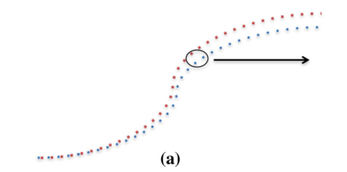
\includegraphics[scale=1.0]{figure2.png}
\caption{Figura 2. Výsledky hráča a simulovaneho vodiča}
\end{figure*}
\section{Zhodnotenie}

\bibliography{literatura}
\bibliographystyle{plain} % prípadne alpha, abbrv alebo hociktorý iný
\end{document}

